\documentclass{article}

\usepackage[utf8x]{inputenc}
\usepackage[english,russian]{babel}
\usepackage{graphicx}
\usepackage{amsmath}
\usepackage{amssymb}
\usepackage{extarrows}
\usepackage{vmargin}
\usepackage{MnSymbol}
\setpapersize{A4}
\setmarginsrb{2cm}{2cm}{2cm}{2cm}{0pt}{0mm}{0pt}{13mm}
%\usepackage{cmap}


\begin{document}

\centerline{\large Курс лекция для магистров ВМК МГУ}
\centerline {\textbf{\LARGE Обратные задачи математической физики}}
\centerline {Затехал Строков Вениамин 2025}

\vspace{0.4cm}

\centerline{\LARGE Лекция 1. Математические модели естествознания и обратные задачи}

\vspace{0.5cm}

Математическая физика изучает явления окружающей природы в рамках точных математических постановок на основе познанных закономерностей.
Основой такого изучения являются математические модели.

Математическую физику характеризует то, что на основе установленных закономерностей возможна постановка задач, замкнуто описывающих исследуемый процесс или явление.

В рамках математической физики основным объектом изучения являются причинно-следственные связи и их последствия.

$$ Z \xLongrightarrow{\text{A}} U $$

Причина Z, закономерность A, следствие U - это математическая модель \textit{прямой задачи} (ПЗ, PD)

Прямые задачи характеризуют (как правило):\\
1) однозначность результата,\\
2) непрерывная зависимость U от Z;\\
при задании достаточного объёма дополнительных условий, например, начальных, краевых и т.п. Это приводит к возможности детерминированного описания мира (концепция детерминизма).

\bigskip

Рассмотрим теперь класс задач, в которых по следствию определяется причина:

$$ U \xLongrightarrow{\text{R}} Z $$

Следствие U, формальная связь R, причина Z - это математическая модель \textit{обратной задачи} (ОЗ).

Некоторые свойства ОЗ:\\
1) ОЗ физически не реализуемы;\\
2) ОЗ возникают при исследовании объектов и явлений недоступных непосредственному изучению (геофизика, астрономия, радиолокация, неразрушающая диагностика в медицине, технике, физика микромира, и т.д.)\\
3) отсутствие устойчивости, т.е. нет непрерывной зависимости от данных наблюдений, измерений и т.п.

\bigskip

\textbf{Пример 1}. ОЗ рассеяния для стержня

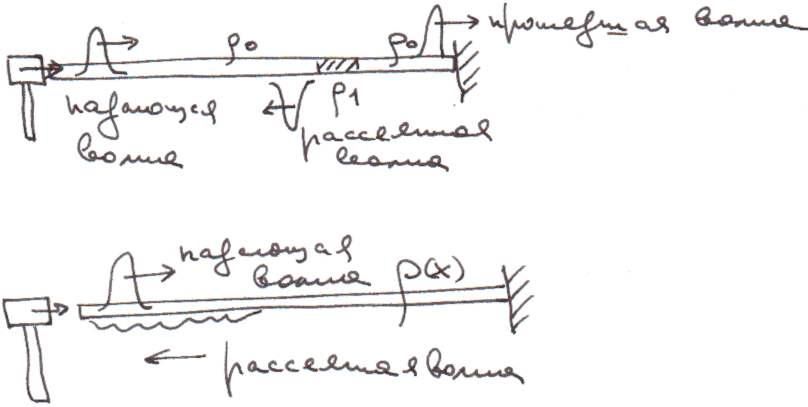
\includegraphics[scale=0.85]{example1.png}

$\phi (t)$ - импульсы воздействия при $x = 0$,

$f(t)$ - измеряемые колебания при $x = 0$,

$\rho(x)$ - неизвестная плотность.

ОЗ рассеяния - найти неоднородность в стержне т.е. найти $\rho(x)$

\newpage

\textbf{Пример 2}. Обратная динамическая задача сейсмики

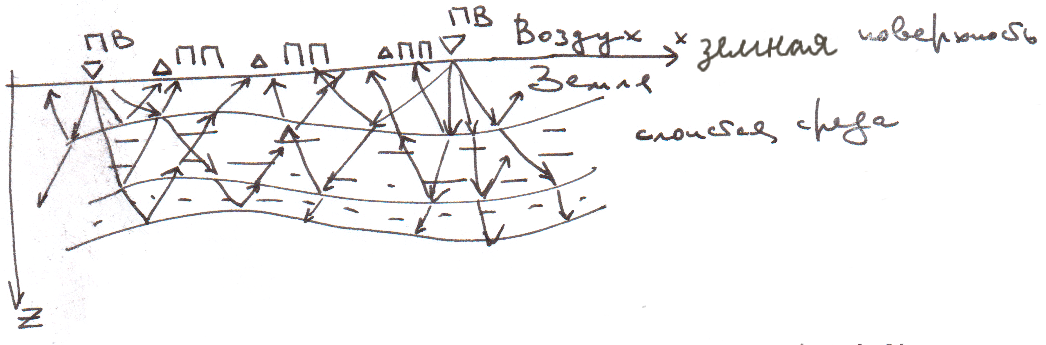
\includegraphics[scale=0.75]{example2.png}

$z = \phi_j(x)$ - уравнения границ

$\rho_j(x)$ - плотности в слое

ОЗ: по рассеянному полю восстановить среду - т.е определить геологический разрез.

\bigskip

\textbf{Пример 3}. Обратная спектральная задача

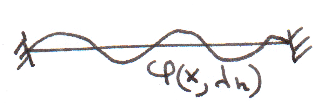
\includegraphics[scale=1]{example3.png}

Имеется струна переменного сечения $S(x)$ и плотности $\rho(x)$, $T = const$

$$ \rho(x) S(x) u_{tt} = T u_{xx}, 0 < x < l. $$

Известны частота собственных колебаний ${\lambda_k}$ и ${\phi'(0,\lambda_k)}$, при $|| \phi(x,\lambda_k)||_{L_2[0,l]}=1$, можно ли определить $\rho(x), S(X)$?

\bigskip

\textbf{Пример 4}. Обратная задача гравиметрии

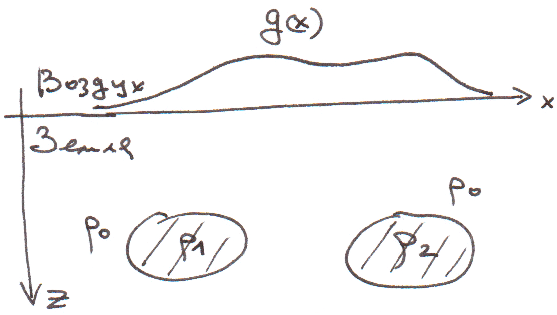
\includegraphics[scale=0.6]{example4_1.png}

$g(x)$ - амплитуда поля тяготения. 

Можно ли определить рудные тела по $g(x)$?

\smallskip
Обратная задача теории потенциала

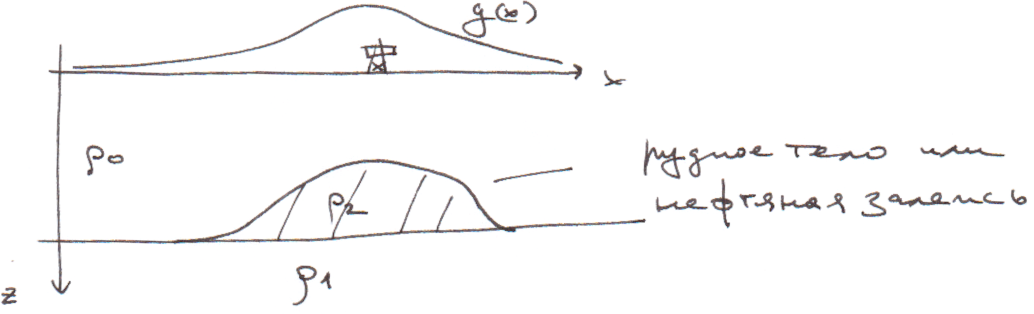
\includegraphics[scale=0.6]{example4_2.png}

Можно ли найти конкретную границу, т.е. форму резервуара или рудного тела?


\bigskip


\centerline{\large Корректная и некорректная задачи}


Итак, $R(u) = z$ - обратная задача. $u$ дано, требуется найти $z$.

Пусть $u \in U$, $z \in Z$, $U,Z$ - некоторые множества, далее метрические пространства.

\smallskip

\textit{Опр. Задача $R(u) = z$ называется корректной по Адамару на $U,Z$ если}

\textit{1) $\forall u \in U$ $\exists z = R(u), z \in Z$,}

\textit{2) решение $z$ единственно,}

\textit{3) $z$ непрерывно зависит от $u$.}


\bigskip
\textbf{Пример 1}. Определение правой части ОДУ.

Пусть $x \in X = C[0,T], f \in F = C[0,T]$.
$$
\begin{cases}
x''(t) = f(t), \hspace{1cm} 0 \leqslant t \leqslant T;\\
x(0) = x'(0) = 0.
\end{cases}
$$ 
Задача определения $f(t)$ по $x(t)$ является некорректной.
Решение единственно, если существует, но оно существует не для $\forall x \in X$.
Устойчивость отсутствует, например для:\\
$$
x_n = \frac{1}{n} sin(n^2t) \rightarrow 0, n \rightarrow \infty ,
$$

$f_n$ - расходится при $n \rightarrow \infty $

Задача становится корректной при $X = C^2[0,T]$.

\bigskip

Замечание 1. Если отображение $R$ - линейно, то достаточно исследовать единственность и устойчивость нулевого решения.

Замечание 2. Задаче $R(x) = f$ можно сопоставить эквивалентную задачу решения операторного уравнения $Af = x$, где

$$
Af = \int_0^t (t - \tau) f(\tau) d \tau = x(t), \hspace{1cm} 0 \leqslant t \leqslant T.
$$

\bigskip

\textbf{Пример 2}. Интегральное уравнение Фредгольма I рода:

$$
Az = \int_a^b K(x,s) z(s) ds = u(x),  \hspace{1cm} x \in [c,d],
$$
При $K \in C([c,d] \times [a,b])$ эта задача некорректна.
Покажем это на отрезке $[0,\pi]$:

Пусть $Az_0 = u_0$ и $z_n^{(s)} = z_0^{(s)} + N \sin (ns)$.

$$
u_n(x) - u_o(x) = N \int_0^{\pi} K(x,s) sin(ns) ds = N K_n(x),  \hspace{1cm} c \leqslant x \leqslant d,  
$$
где $K_n(x)$ - коэффициенты Фурье $K(x,s)$ по переменным $s$.

Покажем, что $K_n \rightrightarrows 0$ при $n \rightarrow \infty $.

1) Нетрудно проверить, что $K_n(x) \in C[c,d]$ и $|K_n(x)| < M$, $\forall n \in \mathbb{N}$.\\

2) Последовательность $K_n(x)$ равно степенно непрерывна, поскольку $K_n(x)$ непрерывна и $\Rightarrow$ равномерно непрерывна на $[c,d] \times [a,b]$, 
т.е. существует $ \omega(h) \rightarrow 0 $ : 
$$
|K(x',s') - K(x'',s'')| \leqslant \omega ((x' - x'') + (s' - s'')).
$$ 
Тогда 
$$
|K_n(x') - K_n(x'')| \leqslant \int_0^{\pi} |K(x',s) - K(x'',s)| sin (ns) ds \leqslant \pi \omega (|x' - x''|),
$$
$w(h)$ - модуль непрерывности.

По теореме Арцела $\exists K_{n_p}(x) \rightrightarrows 0$ при $p \rightarrow \infty $ $\Rightarrow$ и вся $K_n(x) \rightrightarrows 0$ при $n \rightarrow \infty $.
 Т.о. $\exists \varepsilon(n) > 0, \varepsilon (n) \rightarrow 0, n \rightarrow \infty $: $|K_n(x)| \leqslant \varepsilon(n)$

Выберем теперь $N = N(n)$ так, что $N(n) \rightarrow 0$ и $N(n)\varepsilon(n) \rightarrow 0$ при $n \rightarrow \infty $ ( например $N(n) = \frac{1}{\sqrt{\varepsilon (n)}}$)

Тогда 
$$
z_n(s) - z_0(s) = \frac{1}{\sqrt{\varepsilon (n)}} \sin(ns)
$$
и 
$$
\max_{[0,\pi]}[z_n(s) - z_0(s)| = \frac{1}{\sqrt{\varepsilon (n)}},
$$ 
но $|u_n(x) - u_0(x)| \leqslant \sqrt{\varepsilon (n)}$ $\Rightarrow$ решение неустойчиво, т.е. нет непрерывной зависимости решения от правой части.

\textbf{Пример 3}. (Адамара)

Найти $z(x,y)$ : 
$$
\begin{cases} 
z_{xx} + z_{yy} = 0, \hspace{3cm} x \in \mathbb{R}, 0 < y \leqslant b;\\

z(x,0)=0, z_y(x,0) = u(x), \hspace{1cm} x \in \mathbb{R}.
\end{cases}
$$

Введём для $z(x,y)$ и $u(x)$ равномерные метрики. Тогда задача $z = R(u)$ - некорректна. Действительно, для $ u_n(x) = \frac{1}{n} sin(nx) \rightarrow 0, n \rightarrow \infty $ существует единственное решение.

$$
z_n(x,y) = \frac{1}{n^2} \sin(nx) \sh(ny) \nrightrightarrows 0
$$ 
Например, при $x_n = \frac{\pi}{2n}, y =1$, $z_n(x_n, 1) \rightarrow \infty $ при $n \rightarrow \infty $


\end{document}